% ============================================================
% 1.1 INTRODUCTION: STUDENTS' BACKGROUNDS -- Writer: Ignacio Gimeno
% Target: about 280 words + Figure 1 (student background by degree). The Introduction is split in three files: 01a (Ignacio), 01b (Adam), 01c (Ignacio).
% Brief: "Introduction, including Background and Related Work: research
% question, motivation, dataset significance, objectives, and the relevant
% scientific or technical background and prior work ... integrated into the
% Introduction rather than submitted as a separate chapter."
% IRENE'S FEEDBACK ON THE SENTENCE OUTLINE (follow it in this order):
%   "Begin with how students' backgrounds can shape their choice of degree,
%    then explain why GPA comparisons across fields raise a fairness question."
%   "expand the literature beyond the current five references"
%   "use graphs to help readers understand the analysis ... interpret the visuals"
%   "Use first-person plural consistently to describe your work"
% Template: avoid a broad textbook opening; every objective must connect to a
% result and a conclusion; signpost the report without listing section titles.
% All references below were checked (Crossref) and are in 90_works_cited.tex.
% ============================================================

\subsection{Students' Backgrounds and the Choice of Degree}
\label{sec:context}

\guide{Ignacio -- Paragraph 1: background shapes the choice of degree (literature)}{%
\textbf{Establish (Irene):} the degree a student enters is not random: family background, gender, preferences and prior achievement shape it.\\
\textbf{Sources (MLA in-text):} family socioeconomic status and parental involvement are linked to the choice of major, with differences by gender, ethnicity and nativity (Ma); the gender gap in majors is explained mainly by preferences and tastes rather than by expected ability (Zafar); students sort into majors by ability (Arcidiacono); review of how school curriculum and major choice differ across students and shape careers (Altonji et al.). Compare them in two or three sentences; do not list them.}
\budget{140}{Ignacio}

\guide{Ignacio -- Paragraph 2: our own data show it (Figure~\ref{fig:background})}{%
\textbf{Interpret the figure (Irene: interpret the visuals):} in the 3,703 Portuguese students, the share with at least one parent holding a higher-education degree ranges from 7\% (Social Service, evening) to 50\% (Equinculture), scholarship holders from 8\% (Equinculture) to 42\% (Social Service), women from 2\% (Informatics Engineering) to 95\% (Basic Education); all differences between degrees are far larger than chance ($\chi^2$ tests, 14 df, $p<10^{-25}$; entry grade ANOVA $F = 12.6$, $p < 10^{-28}$). Across the 15 degrees, mean GPA is higher where more students have a graduate parent ($r = 0.40$) and stronger entry grades ($r = 0.44$).\\
\textbf{Why it matters for the question:} degrees differ in who enters them, so a pooled GPA ranking compares students from different backgrounds \emph{and} different grading practices -- the report separates the second from the first as far as the data allow (\S\ref{sec:res-confounders}).\\
\textbf{Source:} \texttt{results/background\_stats.json}, \texttt{results/background\_by\_degree.csv}. Descriptive only: no causal claim.}
\budget{140}{Ignacio}

\begin{figure*}[t]
  \centering
  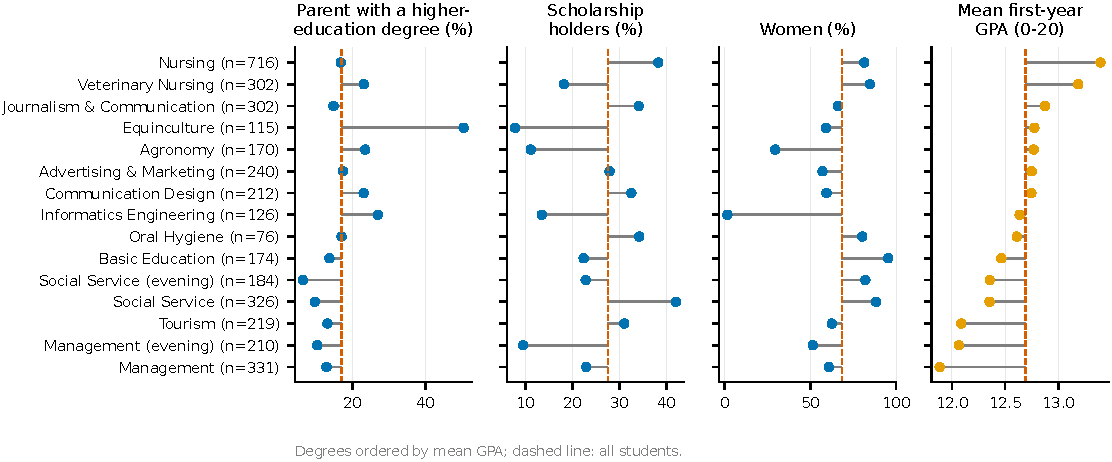
\includegraphics[width=\textwidth]{fig9_background}
  \caption{\capguide{Ignacio -- what is shown (background of the students of each degree, 15 degrees, 3,703 students of one Portuguese polytechnic, cohorts 2008--09 to 2018--19); definition of ``parent with a higher-education degree'' (mother or father with a completed bachelor's, master's or doctorate); degrees ordered by mean first-year GPA; dashed line = all students; source (Realinho et al.).}}
  \label{fig:background}
\end{figure*}

